\documentclass[11pt, letterpaper, twoside]{article}
\usepackage[utf8]{inputenc}
\usepackage[T1]{fontenc}
\usepackage{fancyhdr}
\usepackage[margin=1in, include foot]{geometry}
\usepackage{ragged2e}
\usepackage[]{hyperref}
\usepackage{apacite}
\usepackage{setspace}
\usepackage[labelformat=empty]{caption}
\usepackage{subcaption}
\usepackage{etoolbox}
\usepackage{graphicx}
\usepackage{amsmath, amssymb}
\usepackage{cleveref}
\usepackage{wrapfig}
\usepackage{afterpage}
\usepackage{floatrow}
\usepackage{tikz}
\usepackage{booktabs}
\usepackage{siunitx}
\usepackage{dcolumn}
\usepackage{pdflscape}
\usepackage{adjustbox}
\usepackage{tablefootnote}
\usepackage{multicol}
% \usepackage{showframe}


\setlength{\parindent}{0pt}
\floatsetup[table]{capposition=top}

\title{\singlespacing\textit{Capitalisn't}: WMATA Advertising Campaign Analysis}


\author{
   Utsav Gandhi
   \and
   Joshua Levy
}

\date{\today}

\begin{document}
\begin{titlepage}   
    \maketitle
    \thispagestyle{empty}
\end{titlepage}



\newpage
\pagenumbering{arabic}

\section{About \textit{Capitalisn't} and this investigation}
\textit{Capitalisn't} is a podcast hosted by Luigi Zingales sand Bethany McLean about ``the ways capitalism is -- or more often isn't -- working in our world today ... and what we can do to fix it.'' Released on a bi-weekly schedule, the podcast's reach has steadily grown since its inception in December 2017.\\

In order to expand the show's reach, in 2021 the Stigler Center (the sponsoring organization of the podcast) previously engaged in two advertising campaign with The Economist Media Group and Vox Media group to raise the awareness of the show. Previous evaluations of those campaigns, however, were limited by the construction of the advertising campaigns and the limited availability of high-resolution data.\\

Since then, in an effort to more rigorously evaluate the potential effects of advertising on audience size, the Stigler Center has run a more narrowly defined ad campaign with the Washington Metropolitan Area Transit Authority (WMATA). The design of this was varied in space and in time so as to generate plausible exogeneity in ``treatment'' (exposure to advertising). Moreover, with advance notice the resolution of data collection is considerably higher than was previously available. In this investigation, we employ, ordinary least squares (OLS), regression-discontinuity, and difference-in-differences (DiD) estimation methodologies in an effort to assess the effectiveness of the WMATA ad campaign.

\subsection{Advertising campaigns}
In the course of advertising the podcast, the Stigler Center purchased two kinds of advertisements that were displayed in WMATA stations throughout the greater Washington, D.C.-Maryland-Virginia (DMV) metropolitan area and in train cars on the WMATA system. ``Digital'' advertisements were present on digital-signage in stations and ``static'' advertisements were posted in train cars. The digital ads were posted between January 19th, and February 15th, 2023. The static ads were posted between January 16th and February 12th 2023. For purposes of parsimony, we generally refer to the WMATA ad as begin in effect between January 16th and February 15th, 2023, the outer bounds of the two advertisement periods.\footnote{First-hand accounts reveal that many of the static ads were still posted in train cars well after the paid-for campaign period ended. This was the case as late as the end of March, suggesting that estimation methods may be biased due to inaccurate definition of the treatment period. This is addressed at greater length in subsequent sections.} For these two postings, the Stigler Center paid \$40,000.

\subsection{Data summary}
This investigation primarily focusses on the effect of advertising on \textit{downloads} for \textit{Capitalisn't}.\footnote{Because movile internet connectivity has improved considerably since the inception of podcasts, streaming podcasts through third-party services such as YouTube has become an increasingly popular alternative to downloading episodes. We restrict our attention to data made available through the podcast's first-party distribution service, Simplecast, which aggregates streams and downloads across a number of third-party podcast aggregation services. This is not, however, an exhaustive measure of the podcasts's audience.} Simplecast, the first-party distribution service that the Stigler Center uses, provides API endpoints that allow us to query for downloads data at varying degrees of temporal- and entity-resolution. Much of this investigation focusses on episode-daily-level downloads data.\\

Additionally, because of the podcast's bi-weekly release schedule downloads 14- and 28-days following release are of interest. Table \ref{episode-level-summary-stats} presents some cursory summary statistics about cumulative downloads to in these intervals. Two aggregate phenomena are worth explicating. First, note that almost every statistic is lower is lower in the full sample (Panel A) than in the most-recent-20 sample (Panel B) of episodes. This represents a secular growth in the podcast over time whereby the early performance of old podcast episodes (when the podcast was small and hand not yet developed a loyal audience) is considerably poorer than that of recent episodes (which receive many more ``first-day downloads''\footnote{``First-day downloads'' here refers to downloads made while the } due to a steady cohort of regular listeners who have ``subscribed' to the podcast''). This phenomenon is underscored by the performance of the most recent episode. Note that the maximum value of the ``Downloads $t=14$'' statistic is greater than the maximum value of the ``Downloads $t=28$'' statistic. That is, the most recent has already received more downloads in 14 days than the next-best-performing episode did in 28 days (and this episode has not yet been released for 28 days).\\

\begin{table}

\caption{Episode-level Summary Statistics \label{tab:ep-summ-stats}}
\centering
\begin{tabular}[t]{llrrrrrr}
\toprule
  &    & Min & P25 & Mean & Median & P75 & Max\\
\midrule
Back Catalog & Days since release & \num{257} & \num{708} & \num{1128} & \num{1120} & \num{1556} & \num{1962}\\
 & Downloads ($t=14$) & \num{407} & \num{4752} & \num{7622} & \num{7422} & \num{9593} & \num{16225}\\
 & Downloads ($t=28$) & \num{1847} & \num{5295} & \num{8683} & \num{8207} & \num{11092} & \num{18583}\\
Recent 20 & Days since release & \num{12} & \num{66} & \num{120} & \num{110} & \num{176} & \num{243}\\
 & Downloads ($t=14$) & \num{11928} & \num{12994} & \num{14125} & \num{13734} & \num{14536} & \num{19581}\\
 & Downloads ($t=28$) & \num{13303} & \num{14893} & \num{15824} & \num{15413} & \num{16252} & \num{22324}\\
\bottomrule
\multicolumn{8}{l}{\rule{0pt}{1em}Values rounded to nearest integer}\\
\end{tabular}
\end{table}


There are over 150 episodes in the \textit{Capitalisn't} catalog. However, because of the secular growth phenomenon identified above and because of the (im)plausible effect of treatment on episodes ``deep'' in the back-catalog of episodes, much of the analysis is restricted to more recently released episodes --- often to the 50 most recently released episodes, or episodes released since the change of hosts in 2020, for example.

\subsection{Advertising effectiveness}
In short, advertising of the type conducted in the WMATA campaign is ineffective.

\section{Motivating Figures}
Many of the short- and long-run phenomena associated with podcast performance are well summarized by a handful of motivating data visualizations. Consider, for example, Figure \ref{fig:all_1142842_cumul_perf} below. Each of these barbell plots display cumulative downloads 1, 14, 28, and 42 days following release.\footnote{Figure qwer does this for a sample of the 20 most recent recent episodes (and is available in the Appendix), the newest of which may not have been released for sufficiently long for all data points to be available.} Two trends are noteworthy. First, as explicated above, there appears to be a secular growth in the performance of the podcast over time. This is borne out in first-day downloads (supposing that listeners who download the podcast on the day of release are ``die-hard'' listeners who are not particularly swayed by the topic presented in a single episode.)

\begin{figure}[!htbp]
  \centering
  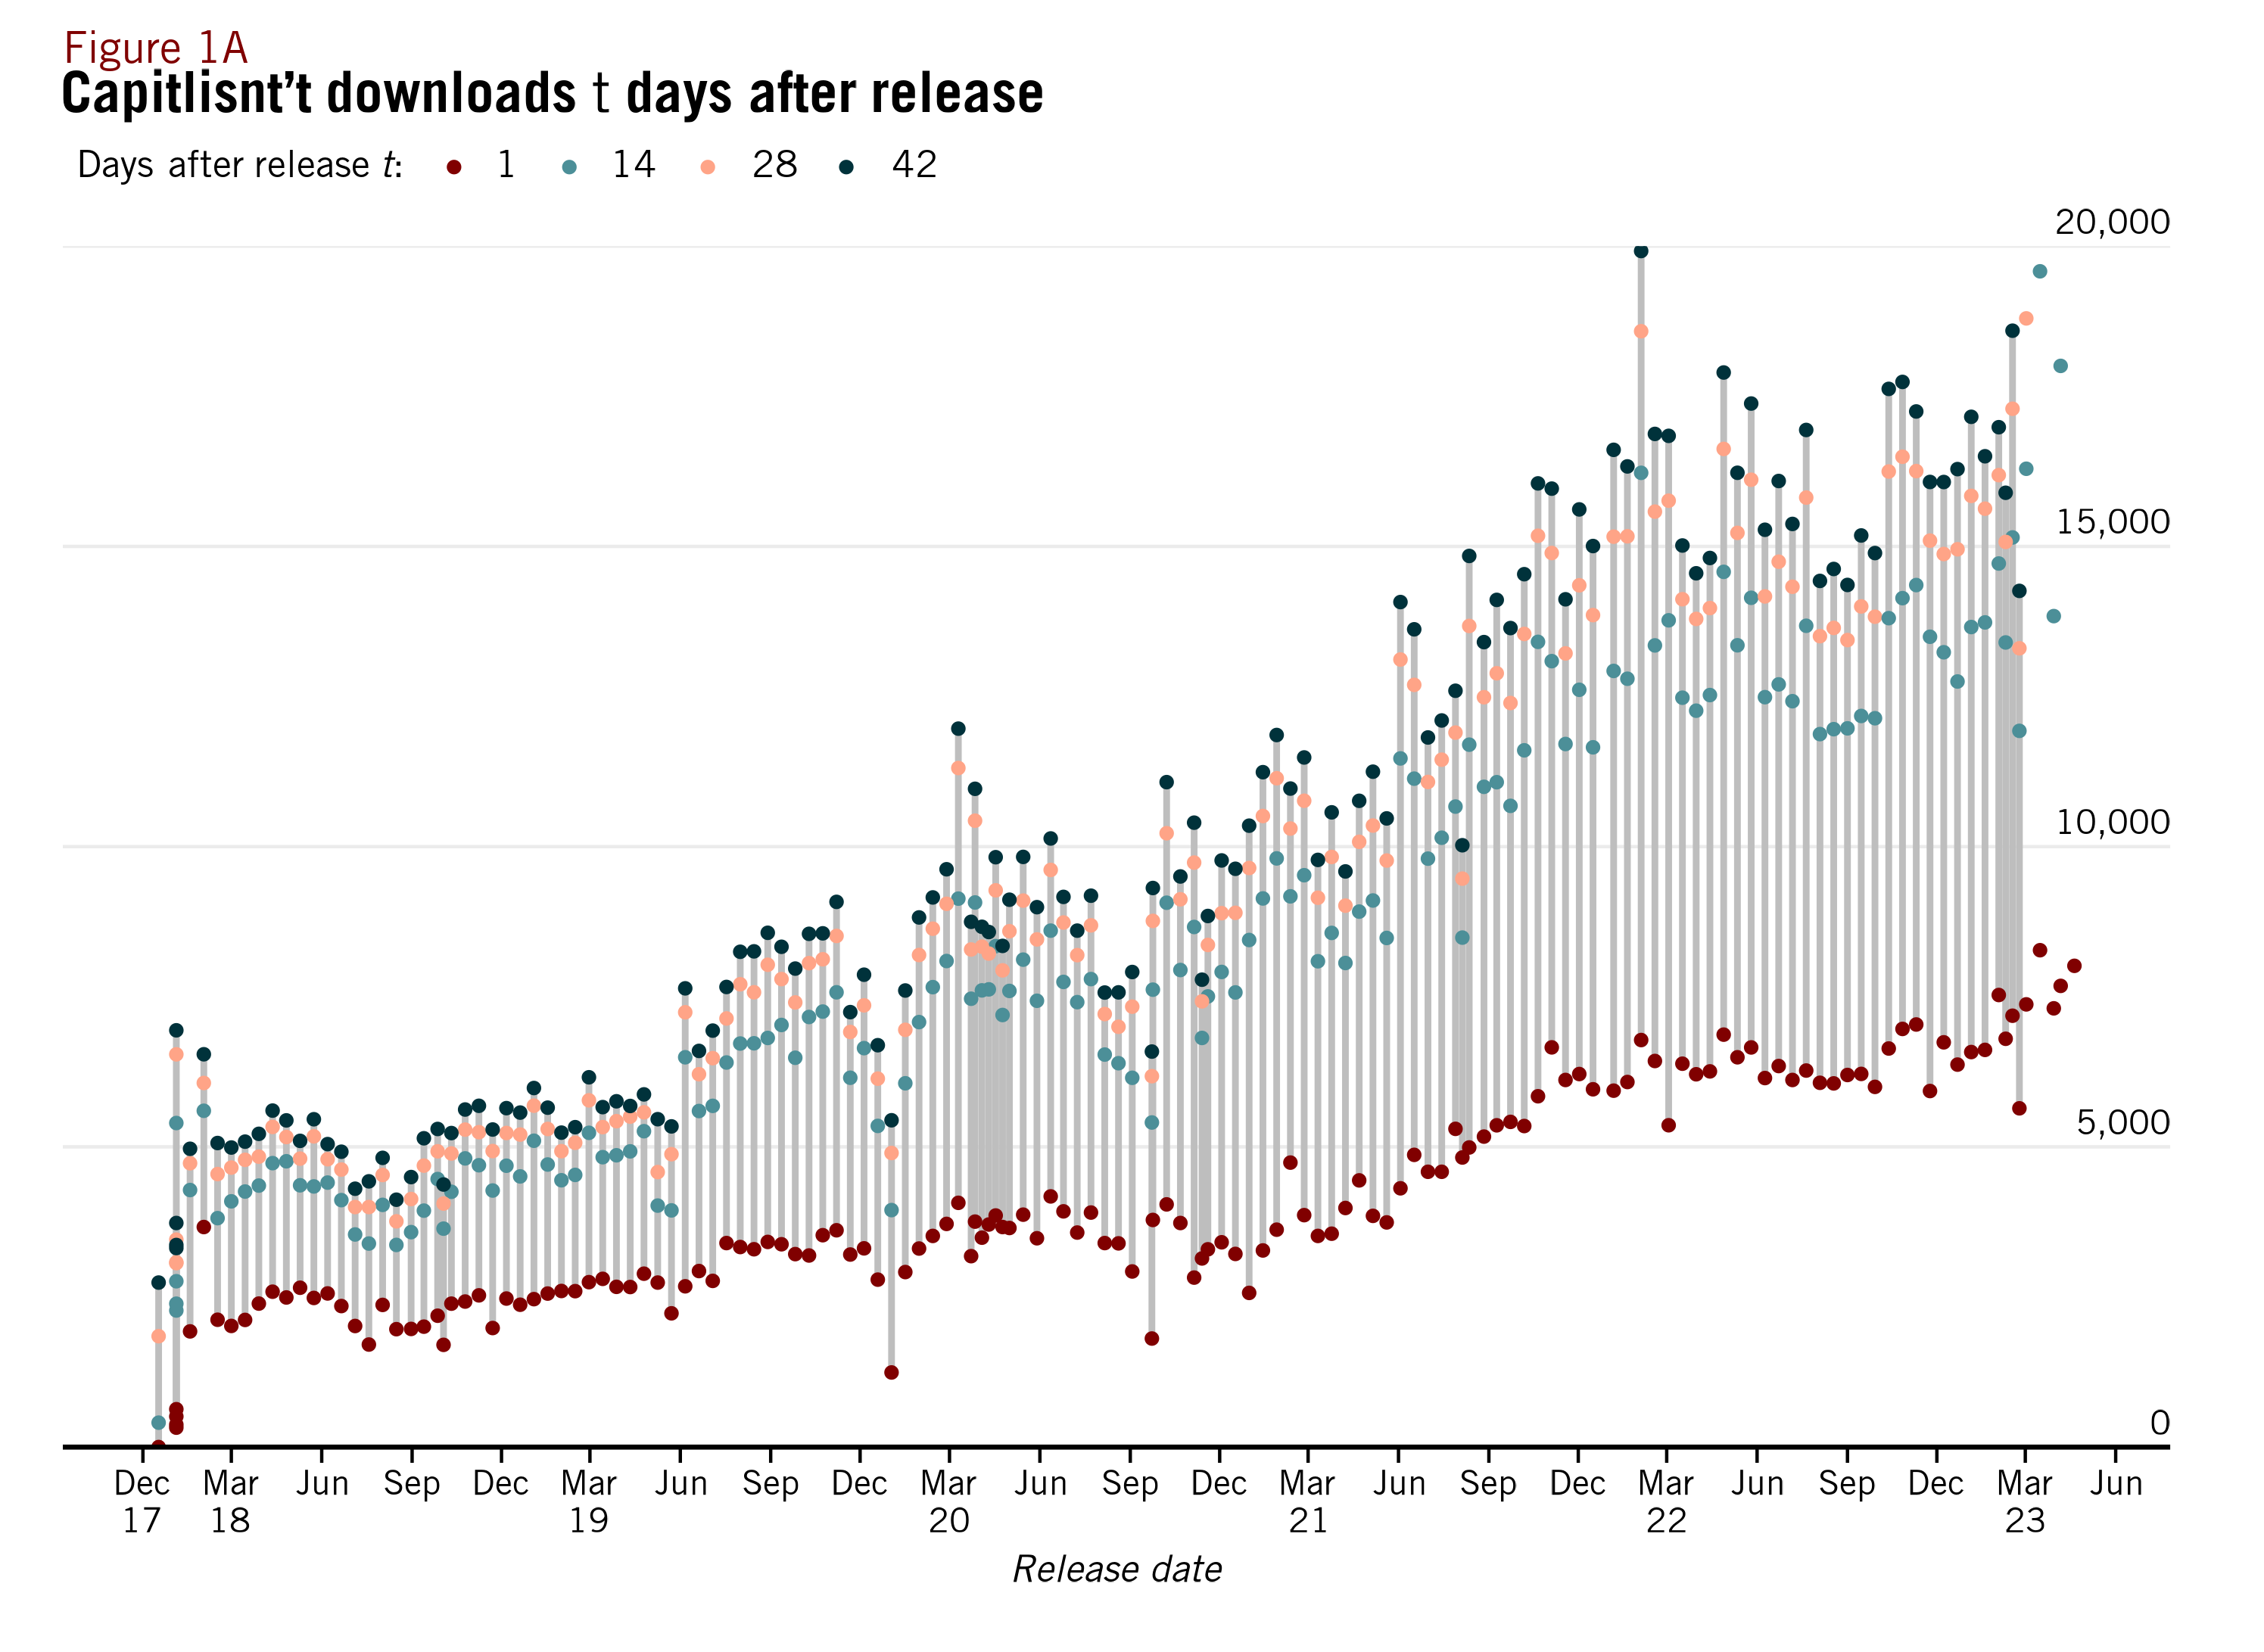
\includegraphics[width=0.9\textwidth]{figures/all_1142842_day_cumul_perf.png}
  \caption{}
  \label{fig:all_1142842_cumul_perf}
\end{figure}

Secondly, and perhaps more importantly, this is also clear in the mid-run performance of new episodes relative to old episodes. That is, even if listeners are not of the die-hard type, there are a growing number of listeners who are ``loyal'' (will eventually get around to the episode even if it isn't their highest priority). Though the logic for identifying the loyal listeners is fuzzier than that for identifying die-hard listeners, a number of mid-run phenomena constitute evidence for their growing number. Consider that for the first year of the podcast's run (between March 2018 and June 2019), the ``tail'' of episode downloads was almost constant as symbolized by the almost flat trend line that would run through all of the blue, 42-day downloads. However, following this period the ``growing'' barbell corresponds to greater gaps between first-, 14-, 28-, and 42-day downloads. These growing gaps suggest that listeners either a) continue to discover the podcast for the first time and listen to the back catalog; or b) have already discovered the podcast in the past, and are of the loyal type and will eventually get around to listening a given episode following its release. The widening of the barbell over time represents a growing loyal audience.\\

\begin{figure}[!htbp]
  \centering
  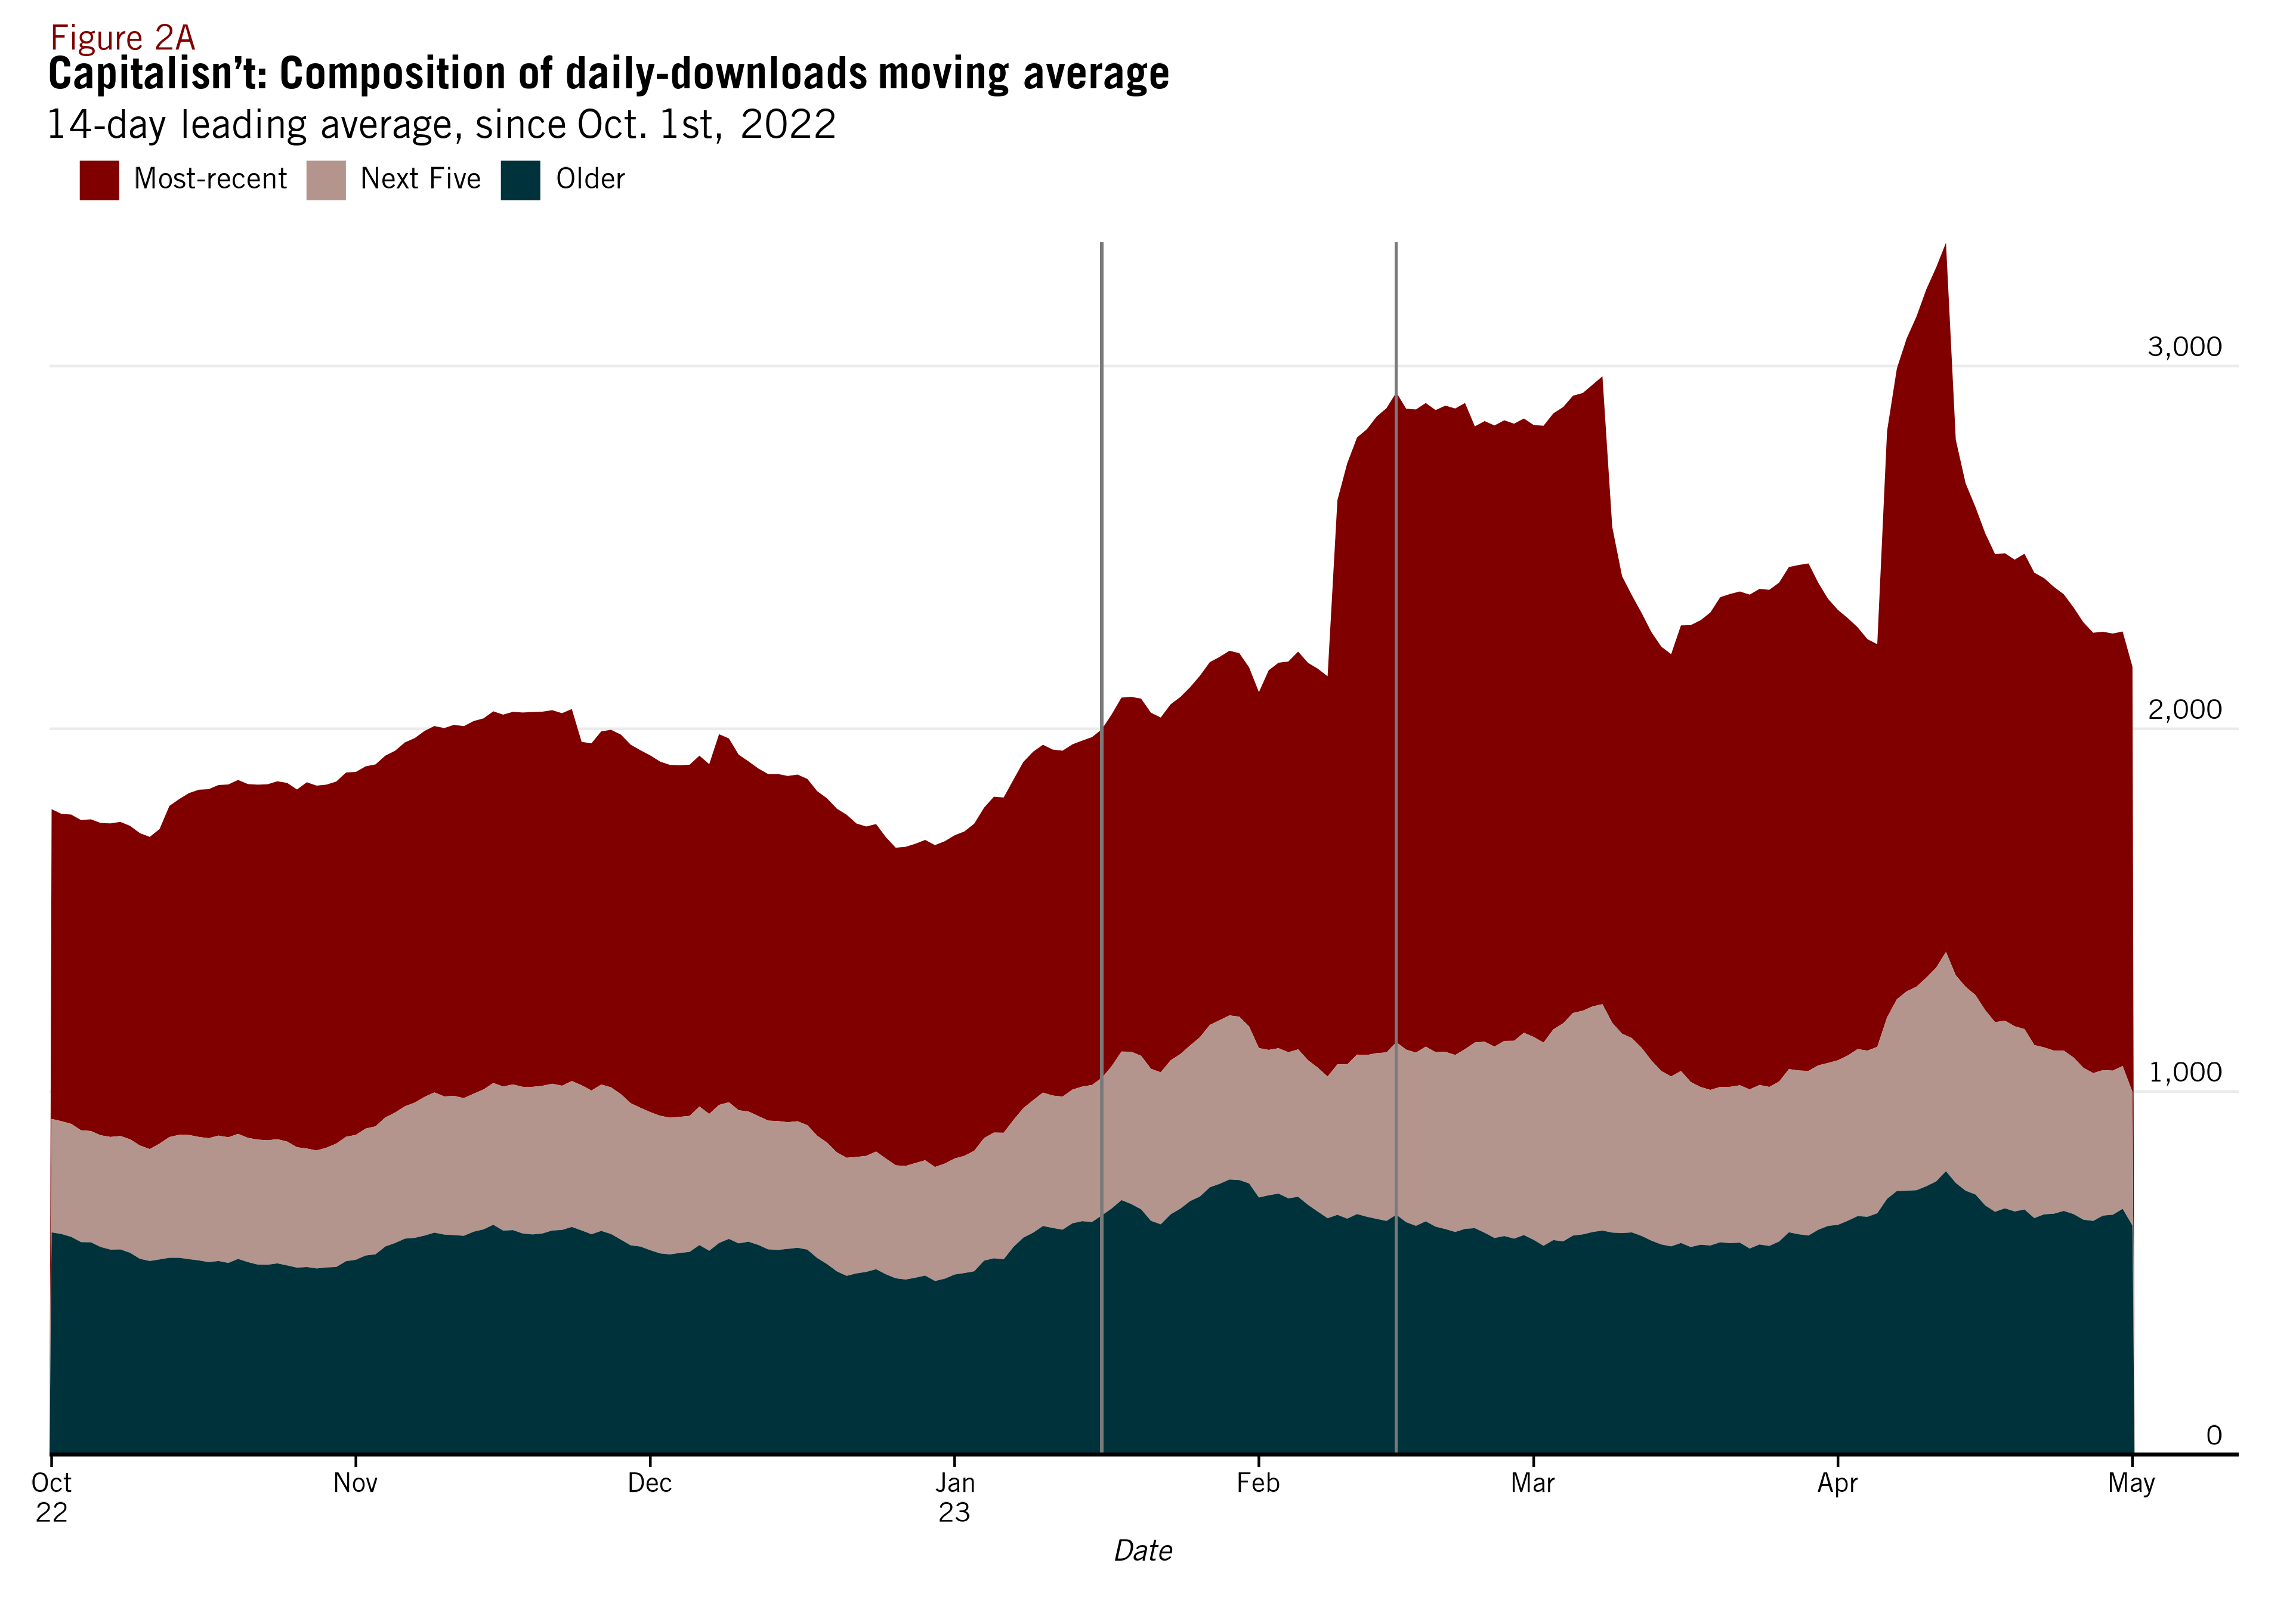
\includegraphics[width=0.9\textwidth]{figures/recent_podcast_moving_avg_decomp.png}
  \caption{}
  \label{fig:recent_moving_avg_perf_decomp}
\end{figure}

\begin{figure}[!htb]
  \centering
  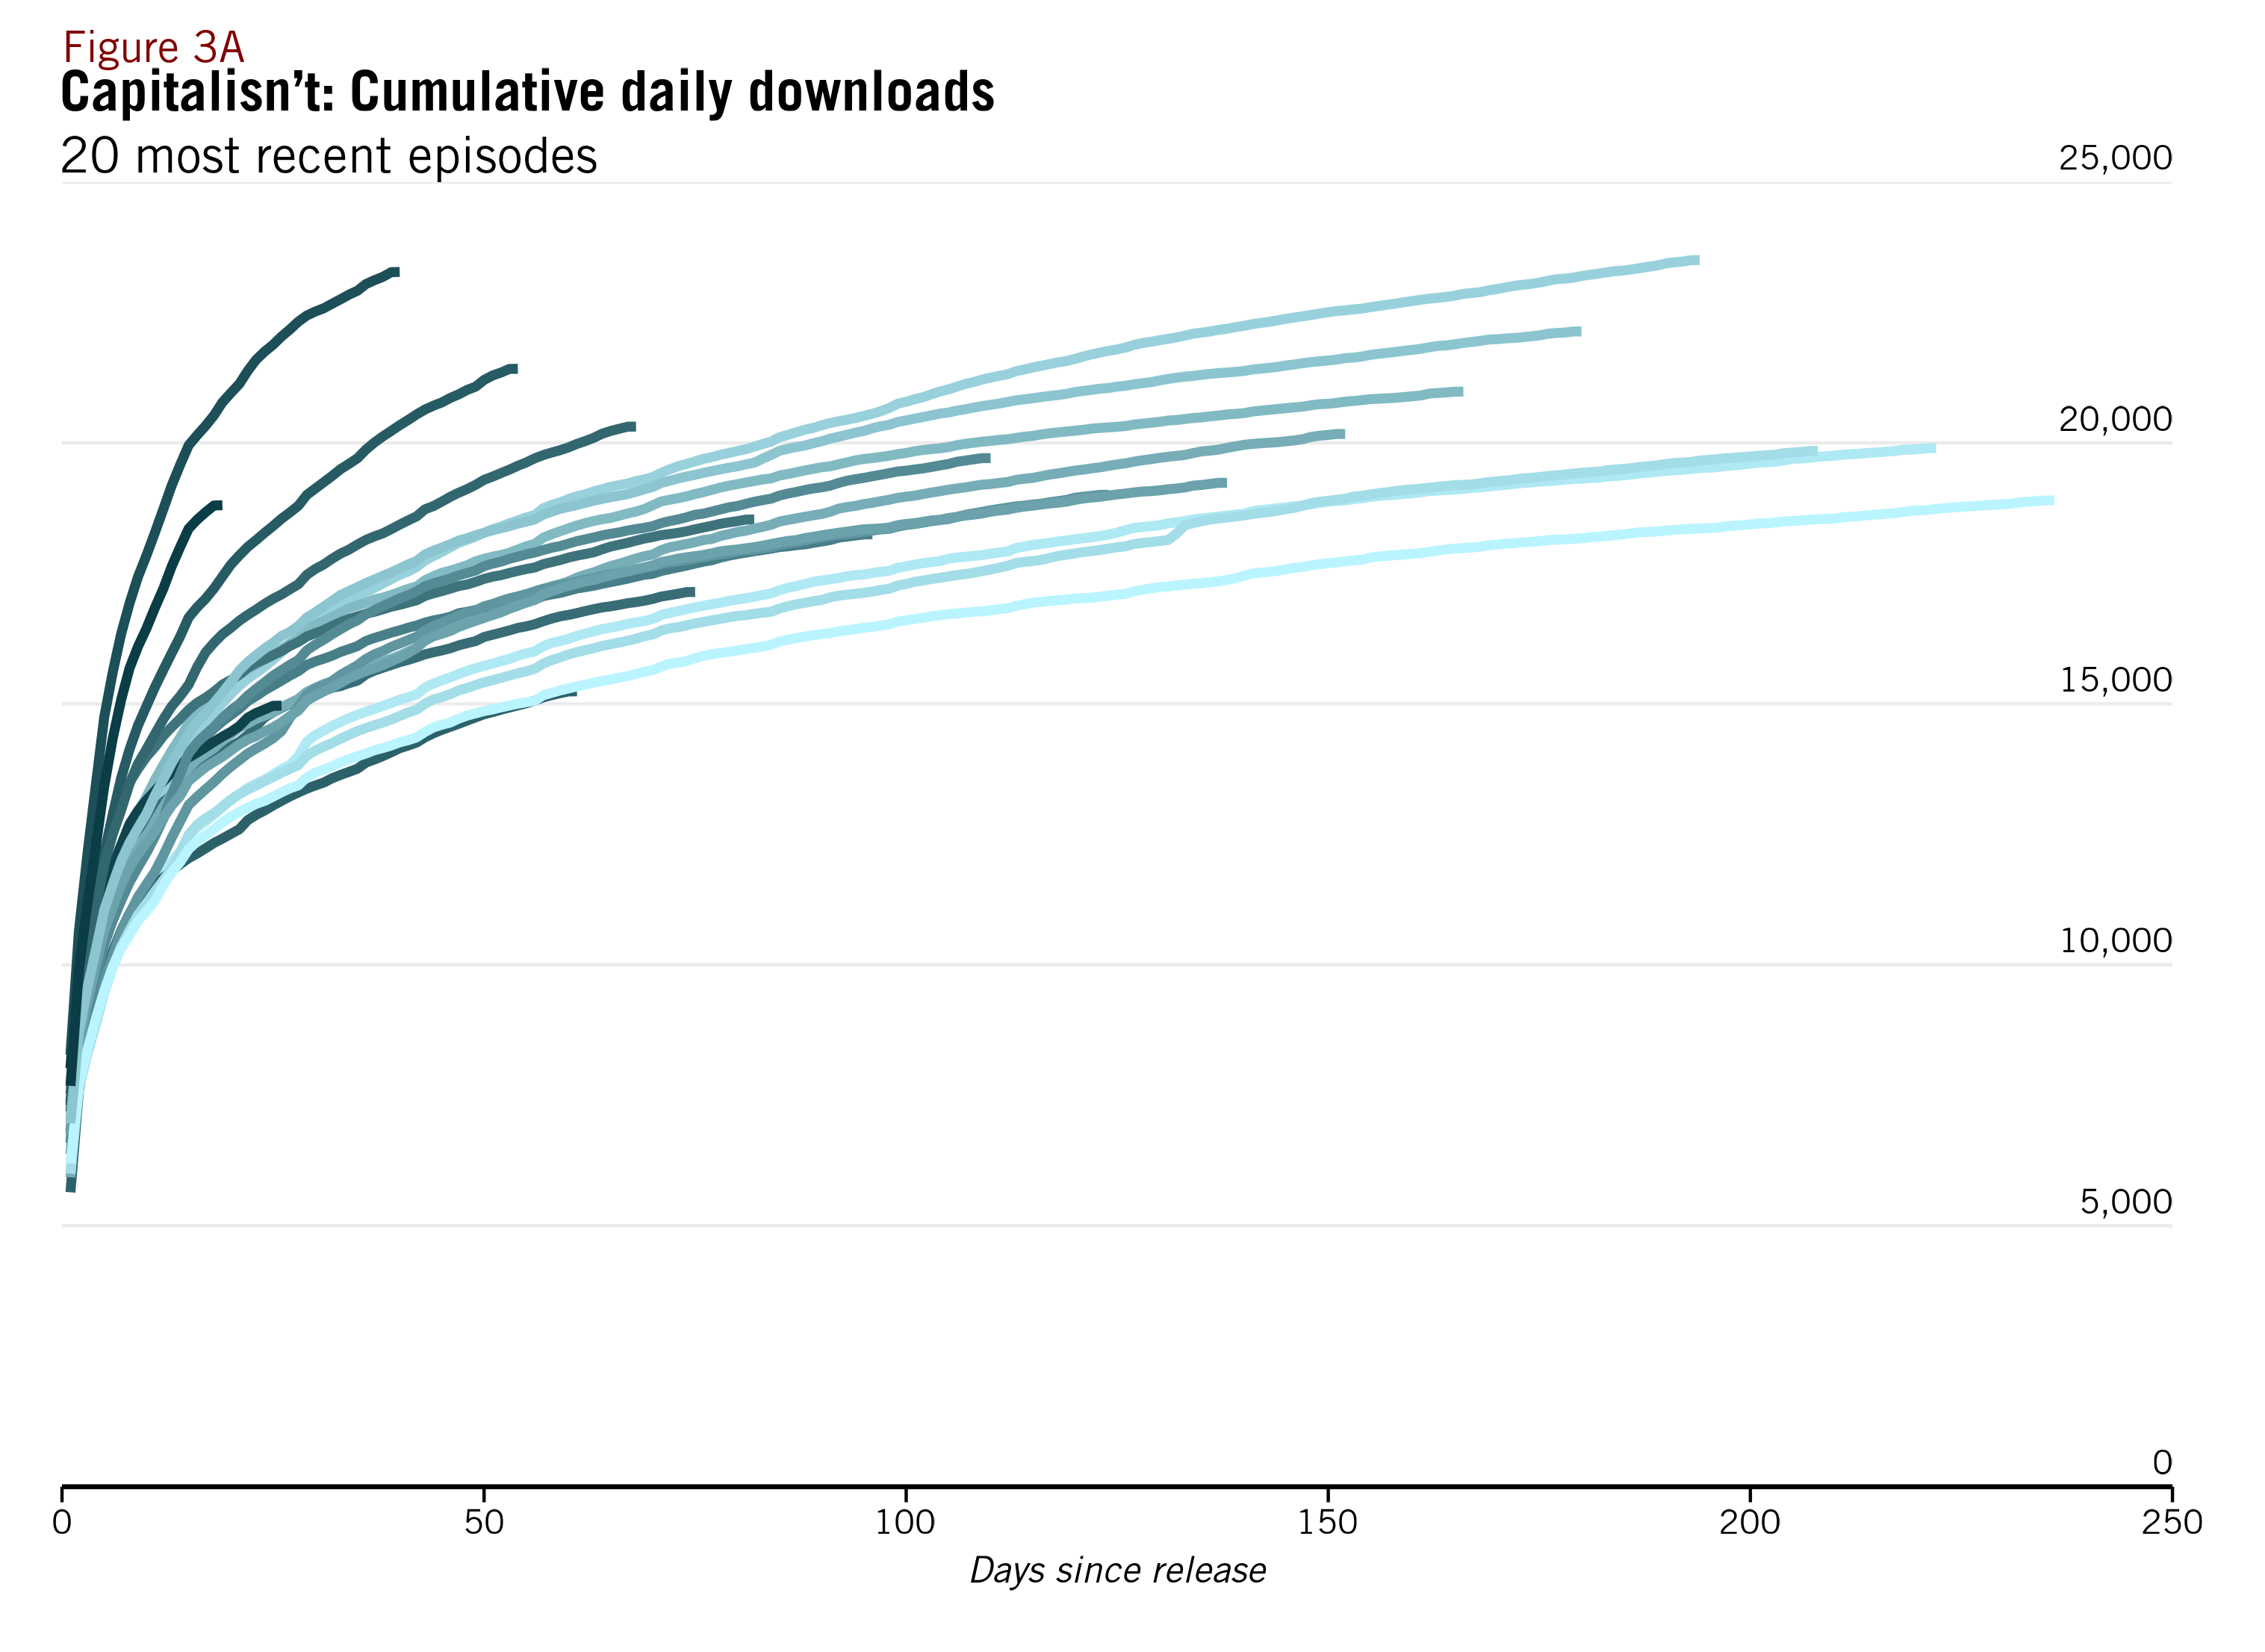
\includegraphics[width=0.9\textwidth]{figures/recent_20_episodes_cumul_perf.png}
  \caption{}
  \label{fig:recent_20_cumul_perf}
\end{figure}

The presence of this ``long-tail'' of downloads is further evidenced by Figures \ref{fig:recent_moving_avg_perf_decomp} and \ref{fig:recent_20_cumul_perf}.\footnote{Full-sample equivalents of these figures are available in the appendix.} In Figure \ref{fig:recent_moving_avg_perf_decomp}, the 14-day leading average --- a statistic selected to try to capture the performance of an episode while it is the most recently released episode for a biweekly release cadence --- of the podcast's cumulative (all episodes) downloads is decomposed into three parts: Most-recent, next five, and older. as expected, on any given day, the most-recently released episode constitutes a majority of downloads. However, the subsequent categories also constitute a non-negligible share of downloads suggesting that people continue to listen to the back-catalog of episodes. Additionally, note that whereas the most-recent episode download performance is relatively volatile due to the performance of \textit{only the current episode}, the performance of the back catalog is smoother.\footnote{This phenomenon is most pronounced during the period in late mid-February through March 2023 because the podcast briefly switched to a weekly release cadence (causing a mechanical increase in the 14-day leading average). The next-five, and older-episode downloads, however, are smoothed over a number of episodes.}\\

Figure \ref{fig:recent_20_cumul_perf} also exhibits the evolving performance of the podcast but at the episode level. Cumulative downloads are plotted on the vertical against days since release on the horizontal. Newer episodes are represented in darker shades of blue. The logarithmic shape of cumulative downloads is to be expected. The ``flattening'' of the curve against the vertical axis, however, represents better first-n-day performance of a given episode and the seemingly higher-valued asymptote that newer episodes' cumulative downloads approach represents a growing audience that consistently listens to the growing back-catalog of episodes.\\

In short, there appears to be a considerable weight of evidence that suggests that \textit{Capitalisn't} is a podcast that is growing over time, independent of paid-for advertising efforts. Thus, against this backdrop of secular growth, paid-for advertising would have to be justified by exceptional returns to expenditure.

\section{Policy Evaluation}
This section will report increasingly well-specified estimates of whether the WMATA advertising campaign had significant effects on the performance of the podcast.

\subsection{Naive Episode-Level OLS}
The most naive specification to test whether the ad campaign has an effect would test for whether cumulative downloads (at some point in time) are higher for episodes that are ``treated'' by the ad campaign than those that are not. An episode-level OLS estimation as decribed above may be specified as follows:

\begin{equation}
  \label{ep-level-naive-ols}
  \text{CumulativeDownloads}_i = \alpha + \beta_1\text{Advertisement}_i + X_i +\varepsilon_i, 
\end{equation}

where for each episode $i$, cumulative downloads would be estimated as a function whether or not an episode has experienced the Advertisement (a binary variable) treatment. Thus, we would expect $\beta_1$, the coefficient of interest, to be positive. In \ref{ep-level-naive-ols} $X_i$ is a vector of episode-level control variables that might also be correlated with cumulative downloads. The results of a series of OLS estimates of the above sepcfication are presented in Table .

\begin{table}
\centering
\begin{tabular}[t]{lcccccccc}
\toprule
\multicolumn{1}{c}{ } & \multicolumn{3}{c}{Cumul Downloads (\$t=14\$)} & \multicolumn{5}{c}{Cumul Downloads (\$t=28\$)} \\
\cmidrule(l{3pt}r{3pt}){2-4} \cmidrule(l{3pt}r{3pt}){5-9}
  & (1) & (2) & (3) & (4) & (5) & (6) & (7) & (8)\\
\midrule
Intercept & \num{21.218} & \num{11.097} & \num{11.249} & \num{-43.399} & \num{-71.892} & \num{-72.869} & \num{-43.399} & \num{-250.048}\\
 & (\num{191.957}) & (\num{195.598}) & (\num{195.661}) & (\num{206.001}) & (\num{209.501}) & (\num{210.012}) & (\num{206.001}) & (\num{206.640})\\
Trailing Avg. ($n=5$, $t=14$) & \num{0.974}*** & \num{0.976}*** & \num{0.977}*** &  &  &  &  & \num{2.564}***\\
 & (\num{0.021}) & (\num{0.022}) & (\num{0.022}) &  &  &  &  & (\num{0.724})\\
WMATA Digital Ad &  & \num{-160.259} & \num{-183.939} &  & \num{-452.936} & \num{-465.267} &  & \\
 &  & (\num{543.339}) & (\num{544.082}) &  & (\num{581.485}) & (\num{583.301}) &  & \\
Economist/Vox Ad &  &  & \num{-392.623} &  &  & \num{-317.218} &  & \\
 &  &  & (\num{412.159}) &  &  & (\num{566.305}) &  & \\
Trailing Avg. ($n=5$, $t=28$) &  &  &  & \num{0.985}*** & \num{0.989}*** & \num{0.990}*** & \num{0.985}*** & \num{-1.246}+\\
 &  &  &  & (\num{0.020}) & (\num{0.021}) & (\num{0.021}) & (\num{0.020}) & (\num{0.631})\\
\midrule
Num.Obs. & \num{147} & \num{147} & \num{147} & \num{146} & \num{146} & \num{146} & \num{146} & \num{146}\\
R2 & \num{0.937} & \num{0.937} & \num{0.937} & \num{0.944} & \num{0.944} & \num{0.944} & \num{0.944} & \num{0.949}\\
R2 Adj. & \num{0.936} & \num{0.936} & \num{0.936} & \num{0.944} & \num{0.944} & \num{0.943} & \num{0.944} & \num{0.948}\\
\bottomrule
\multicolumn{9}{l}{\rule{0pt}{1em}+ p $<$ 0.1, * p $<$ 0.05, ** p $<$ 0.01, *** p $<$ 0.001}\\
\end{tabular}
\end{table}



\begin{landscape}
    \thispagestyle{empty}
    \begin{table}[!htbp] \centering
        \caption{}
        \label{}
      \begin{tabular}{@{\extracolsep{5pt}}lcccccccc} 
      \\[-1.8ex]\hline
      \hline \\[-1.8ex]
       & \multicolumn{8}{c}{\textit{Dependent variable:}} \\
      \cline{2-9} 
      \\[-1.8ex] & \multicolumn{3}{c}{Downloads ($t=14$)} & \multicolumn{5}{c}{Downloads ($t=28$)} \\       
      \\[-1.8ex] & (1) & (2) & (3) & (4) & (5) & (6) & (7) & (8)\\ 
      \hline \\[-1.8ex]
       Trailing Avg. ($n=5, t=14$) & 0.989$^{***}$ & 0.992$^{***}$ & 0.995$^{***}$ &  &  &  &  & 2.706$^{***}$ \\
        & (0.023) & (0.023) & (0.023) &  &  &  &  & (0.837) \\
        Trailing Avg. ($n=5, t=28$) &  &  &  & 0.992$^{***}$ & 0.990$^{***}$ & 0.991$^{***}$ & 0.992$^{***}$ & $-$1.361$^{*}$ \\
        &  &  &  & (0.021) & (0.022) & (0.022) & (0.021) & (0.722) \\ 
        WMATA Ad. &  & $-$290.419 & $-$319.412 &  & 332.015$^{*}$ & 319.679$^{*}$ &  &  \\
        &  & (864.114) & (865.346) &  & (188.934) & (190.788) &  &  \\
        Economist/Vox Ad. &  &  & $-$445.718 &  &  & $-$317.228 &  &  \\ 
        &  &  & (505.206) &  &  & (978.033) &  &  \\
        Constant & $-$82.344 & $-$102.220 & $-$103.856 & $-$91.374 & $-$77.835 & $-$79.192 & $-$91.374 & $-$326.518 \\
        & (189.422) & (191.364) & (191.547) & (191.724) & (196.476) & (196.718) & (191.724) & (230.056) \\  
       \hline \\[-1.8ex]
      Observations & 145 & 145 & 145 & 144 & 144 & 144 & 144 & 144 \\ 
      R$^{2}$ & 0.942 & 0.942 & 0.943 & 0.944 & 0.944 & 0.944 & 0.944 & 0.949 \\
      Adjusted R$^{2}$ & 0.941 & 0.941 & 0.941 & 0.943 & 0.943 & 0.943 & 0.943 & 0.948 \\ 
      \hline
      \hline \\[-1.8ex]
      \textit{Note:}  & \multicolumn{8}{r}{$^{*}$p$<$0.1; $^{**}$p$<$0.05; $^{***}$p$<$0.01} \\
      \end{tabular}
      \end{table}
\end{landscape}    

\subsection{DMV Diff-in-Diff}


\begin{table}[!htbp] \centering 
  \caption{}
  \label{}
\begin{tabular}{@{\extracolsep{5pt}}lcc}
\\[-1.8ex]\hline
\hline \\[-1.8ex]
 & \multicolumn{2}{c}{\textit{Dependent variable:}} \\
\cline{2-3} 
\\[-1.8ex] & \multicolumn{2}{c}{cumulative\_downloads} \\
\\[-1.8ex] & (1) & (2)\\
\hline \\[-1.8ex]
 log\_days\_since\_release & 2,718.561 & 2,718.561$^{***}$ \\ 
  &  & (257.808) \\
  & & \\
 in\_wmata\_general\_ad &  &  \\
  &  &  \\
  & & \\
 log\_days\_since\_release:in\_wmata\_general\_ad &  &  \\
  &  &  \\
  & & \\
 Constant & 8,144.782 & 8,144.782$^{***}$ \\ 
  &  & (228.348) \\
  & & \\
\hline \\[-1.8ex]
Observations & 5 & 5 \\
R$^{2}$ & 0.982 & 0.982 \\
Adjusted R$^{2}$ & 0.976 & 0.976 \\
Residual Std. Error (df = 3) & 267.810 & 267.810 \\
F Statistic (df = 1; 3) & 166.468$^{***}$ & 166.468$^{***}$ \\ 
\hline
\hline \\[-1.8ex]
\textit{Note:}  & \multicolumn{2}{r}{$^{*}$p$<$0.1; $^{**}$p$<$0.05; $^{***}$p$<$0.01} \\
\end{tabular}
\end{table}


\end{document}